% !TEX root = ../projektdokumentation.tex

\section{Projektdurchführung}\label{projektdurchfuxfchrung}

% \section{Entwurfsphase}
% \subsection{Zielplattform}
% \subsection{Architekturdesign}
% \subsection{Entwurf der Benutzeroberfläche}
% \subsection{Datenmodell}
% \subsection{Geschäftslogik}
% \subsection{Maßnahmen zur Qualitätssicherung}
% \subsection{Pflichtenheft/Datenverarbeitungskonzept}

\subsection{Vorgehensmodell}\label{vorgehensmodell}

Für die Projektdurchführung wurde das agile Vorgehensmodell \gls{Scrum} gewählt. Scrum ist ein weit verbreitetes Framework für die agile Softwareentwicklung, das iterative und inkrementelle Prozesse unterstützt. Es besteht aus festen Rollen, Ereignissen und Artefakten, die bei der iterativen Softwareentwicklung unterstützen.

Die Entscheidung für Scrum wurde aus mehreren Gründen getroffen. Erstens ermöglicht Scrum eine flexible und anpassungsfähige Entwicklung, die besonders nützlich ist, wenn sich Anforderungen im Laufe des Projekts ändern können. Zweitens fördert Scrum eine enge Zusammenarbeit und kontinuierliche Kommunikation im Team, was zu einer besseren Koordination und höherer Produktivität führt. Drittens erleichtert die iterative Natur von Scrum eine regelmäßige Überprüfung und Anpassung des Projekts, was zu einer höheren Qualität des Bot-Framework geführt hat.

Der Methodologie von Scrum folgend wurde das Projekt in drei Sprints unterteilt, wobei jeder Sprint eine feste Dauer von vier Wochen hatte. Dies ermöglichte es dem Team, sich auf kurzfristige Ziele zu konzentrieren und regelmäßig Fortschritte zu präsentieren. Die in unserem Fall wöchentlichen Stand-up-Meetings (Daily Scrum) förderten die Transparenz und halfen dabei, Hindernisse schnell zu identifizieren und zu beseitigen. Durch die Sprint Reviews konnte kontinuierlich Feedback vom ganzen Team eingeholt und in die nächste Planungsphase integriert werden. Insgesamt führte der Einsatz von Scrum zu einer besseren Planbarkeit, höheren Flexibilität und einer kontinuierlichen Verbesserung der Projektarbeit.

\subsection{Umsetzung}\label{umsetzung}

\subsubsection{Klassenmodell}\label{klassenmodell}

Das Klassenmodell unserer Anwendung wurde unter Verwendung der Unified
Modeling Language (UML) erstellt. Es zeigt die wichtigsten Klassen, ihre
Attribute und Methoden sowie die Beziehungen zwischen den Klassen.

Zu den Hauptklassen gehören:

\begin{itemize}
\item
  \texttt{User}: Repräsentiert einen Benutzer der Anwendung mit
  Attributen wie \texttt{id}, \texttt{username}, \texttt{password} und
  \texttt{roles}.
\item
  \texttt{Plugin}: Repräsentiert ein Plugin mit Attributen wie
  \texttt{id}, \texttt{name}, \texttt{description} und \texttt{enabled}.
\item
  \texttt{Server}: Repräsentiert einen Discord-Server mit Attributen wie
  \texttt{id}, \texttt{name}, \texttt{owner} und \texttt{plugins}.
\end{itemize}

Die Beziehungen zwischen den Klassen sind durch Assoziationen,
Aggregationen und Kompositionen gekennzeichnet. Zum Beispiel hat die
Klasse \texttt{Server} eine Aggregation von \texttt{Plugin}, was
bedeutet, dass ein Server mehrere Plugins haben kann, aber ein Plugin
ohne einen Server existieren kann.

\begin{figure}[!h]
  \centering
  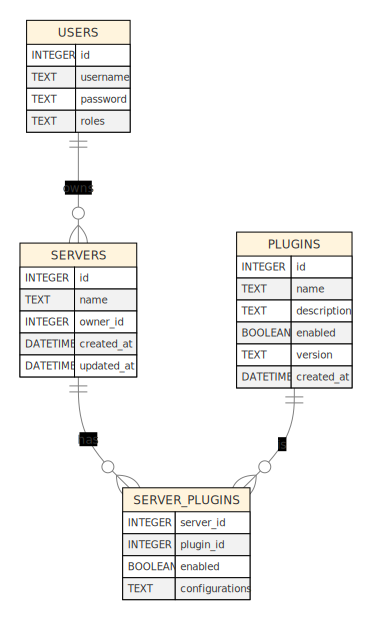
\includegraphics[width=0.8\textwidth]{images/database-diagram-2024-05-27.png}
  \caption{Klassenmodell}\label{fig:klassenmodell}
\end{figure}

\subsubsection{Datenhaltung}\label{datenhaltung}

Für die Datenhaltung wurde eine relationale PostgreSQL-Datenbank erstellt. Die Datenbank enthält Tabellen für Benutzer, Server, Plugins und andere Entitäten.

\begin{itemize}
  \item
        Wahl der Datenhaltung:
  \item
        Beschreibung der Datenbankstruktur und des Datenbankmodells
\end{itemize}

\subsubsection{Design Patterns}\label{design-patterns}

\begin{itemize}
  \item
        Einsatz von Design Patterns:
  \item
        Welche Design Patterns werden verwendet und warum?
\end{itemize}

\subsection{Qualitätssicherung}\label{qualituxe4tssicherung}

\subsubsection{Teststrategien}\label{teststrategien}

\begin{itemize}
  \item
        Beschreibung der Teststrategien:
  \item
        Welche Tests werden durchgeführt (Unit Tests, Integrationstests, Systemtests)?
\end{itemize}

\subsubsection{Testfälle}\label{testfuxe4lle}

\begin{itemize}
  \item
        Konkrete Testfälle:

        \begin{itemize}

          \item
                Beschreibung der durchgeführten Testfälle und deren Ergebnisse
        \end{itemize}
\end{itemize}